\documentclass[10pt,a4paper, margin=1in]{article}
\usepackage{fullpage}
\usepackage{amsfonts, amsmath, pifont}
\usepackage{amsthm}
\usepackage{graphicx}

\usepackage{geometry}
 \geometry{
 a4paper,
 total={210mm,297mm},
 left=10mm,
 right=10mm,
 top=10mm,
 bottom=10mm,
 }

\usepackage{float}
\usepackage{tkz-euclide}
\usepackage{tikz}
\usepackage{pgfplots}
\pgfplotsset{compat=1.13}


\usepackage{geometry}
 \geometry{
 a4paper,
 total={210mm,297mm},
 left=10mm,
 right=10mm,
 top=10mm,
 bottom=10mm,
 }
 % Write both of your names here. Fill exxxxxxx with your ceng mail address.
 \author{
  BAYKARA, Azad\\
  \texttt{e2171320@ceng.metu.edu.tr}
  \and
  KOCAMAN, Alper\\
  \texttt{e2169589@ceng.metu.edu.tr}
}
\title{CENG 384 - Signals and Systems for Computer Engineers \\
Spring 2018-2019 \\
Written Assignment 1}
\begin{document}
\maketitle



\noindent\rule{19cm}{1.2pt}

\begin{enumerate}

\item 
    \begin{enumerate}
    % Write your solutions in the following items.
    \item %write the solution of q1a
    i) $ |z^2| = z. \bar{z}$ \\
    3(x+yj) + 4 = 2j - (x-yj) \\
    3x+4+3yj=2j-x+yj \\
    (4x+4)+(2y-2)j = 0 \\
    Then x = -1 , y=1. So $ |z^2| = (-1+j).(-1-j) = 1+1 = 2$ \\ \\
    ii)
     
	\begin{figure}[h!]
    \centering
        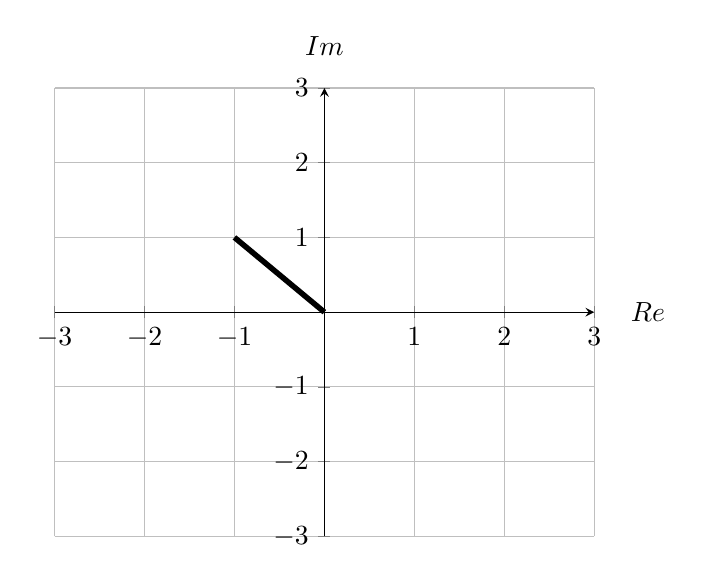
\begin{tikzpicture}[scale=1.0]
           \begin{axis}[
          axis lines=middle,
          xlabel={$Re$},
          ylabel={$Im$},
          xtick={-3, -2, -1, ..., 3},
          ytick={-3, -2, -1, ..., 3},
          ymin=-3, ymax=3,
          xmin=-3, xmax=3,
          every axis x label/.style={at={(ticklabel* cs:1.05)}, anchor=west,},
          every axis y label/.style={at={(ticklabel* cs:1.05)}, anchor=south,},
          grid,
        ]
           \path[draw,line width=2pt] (0,0) -- (-1,1);
           \end{axis}
        \end{tikzpicture}
        \caption{$z = -1 + j$}
        \label{fig:q2}
    \end{figure}   	
   	
    \item %write the solution of q1b
    \begin{align*}
    &z^3 = 4^3.e^{j\frac{\pi}{2}} \\
    &z = 4. e^{j(\frac{\pi}{6} + \frac{2\pi}{3}k)} \ for \ k=0,1,2
    \end{align*}

    \item %write the solution of q1c
    \begin{align*}
    &\frac{\sqrt{2}e^{-j.\frac{\pi}{4}} . 2e^{j.\frac{\pi}{3}}}{\sqrt{2}e^{j\frac{\pi}{4}}} = 2.e^{-j\frac{\pi}{6}} \\
    &Then \ r=2 \ \ \ \theta = -\frac{\pi}{6}
    \end{align*}

    \item %write the solution of q1d
    \begin{align*}
    &-j.(cos(\frac{\pi}{2}) + j.sin(\frac{\pi}{2})) \\
    &= -j.cos(\frac{\pi}{2}) + sin(\frac{\pi}{2}) = 1 \\
    &= 1.e^{j.2\pi}
    \end{align*}
    
    \end{enumerate}


\item %write the solution of q2
Firstly,corresponding t values in $y(t) = x(\frac{1}{2}t+1)$ should be found.\\ 

When t=-2 in $x(t)$ , $\frac{1}{2}t+1 = -2$ $\rightarrow$ $t=-6$ ,\\

When t=-1 in $x(t)$ , $\frac{1}{2}t+1 = -1$ $\rightarrow$ $t=-4$ ,\\

When t= 0 in $x(t)$ , $\frac{1}{2}t+1 =  0$ $\rightarrow$ $t=-2$ ,\\

When t= 1 in $x(t)$ , $\frac{1}{2}t+1 =  1$ $\rightarrow$ $t=-0$ ,\\

When t= 2 in $x(t)$ , $\frac{1}{2}t+1 =  2$ $\rightarrow$ $t= 2$ .\\

In $x(t)$ graph , value from $-\infty$ to -2 (which is 0 ) is value for $y(t) = x(\frac{1}{2}t+1)$ from $-\infty$ to -6 .\\
In $x(t)$ graph , value from $-2$ to $-1$ is value for $y(t) = x(\frac{1}{2}t+1)$ from $-6$ to $-4$ .\\
In $x(t)$ graph , value from $-1$ to $1$ (which is 1) is value for $y(t) = x(\frac{1}{2}t+1)$ from $-4$ to $0$ .\\
In $x(t)$ graph , value from $1$ to $2$ is value for $y(t) = x(\frac{1}{2}t+1)$ from $0$ to $2$ .\\
In $x(t)$ graph , value from $2$ to $\infty$ (which is 0 ) is value for $y(t) = x(\frac{1}{2}t+1)$ from $2$ to $\infty$ .\\

So,the graph of $y(t) = x(\frac{1}{2}t+1)$ is , 

\begin{figure}[h!]
    \centering
        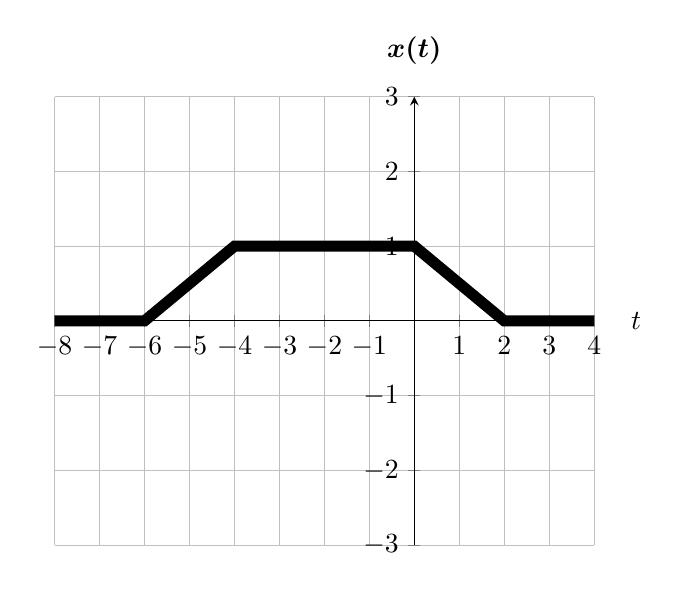
\begin{tikzpicture}[scale=1.0]
           \begin{axis}[
          axis lines=middle,
          xlabel={$t$},
          ylabel={$\boldsymbol{x(t)}$},
          xtick={-8 ,-7,-6, -5,-4, -3, -2, -1, ..., 4},
          ytick={-3, -2, -1, ..., 3},
          ymin=-3, ymax=3,
          xmin=-8, xmax=4,
          every axis x label/.style={at={(ticklabel* cs:1.05)}, anchor=west,},
          every axis y label/.style={at={(ticklabel* cs:1.05)}, anchor=south,},
          grid,
        ]
           \path[draw,line width=4pt] (-8,0) -- (-6,0) -- (-4,1) -- (0,1) -- (2,0) -- (4,0);
           \end{axis}
        \end{tikzpicture}
        \caption{$t$ vs. $x(1/2t+1)$.}
        \label{fig:q2}
    \end{figure}


\item      
    \begin{enumerate}
    \item %write the solution of q3a
This is the graph for x[-n] ,\\
\begin{figure}[H]
    \centering
    \begin{tikzpicture}[scale=1.0] 
      \begin{axis}[
          axis lines=middle,
          xlabel={$n$},
          ylabel={$\boldsymbol{x[-n]}$},
          xtick={ -8,-7,-6,-5,-4,-3,-2,-1, 0,1},
          ytick={-4,-3, -2, -1, ..., 4},
          ymin=-4, ymax=4,
          xmin=-8, xmax=1,
          every axis x label/.style={at={(ticklabel* cs:1.05)}, anchor=west,},
          every axis y label/.style={at={(ticklabel* cs:1.05)}, anchor=south,},
          grid,
        ]
        \addplot [ycomb, black, thick, mark=*] table [x={n}, y={xn}] {q3.dat};
      \end{axis}
    \end{tikzpicture}
    \caption{$n$ vs. $x[-n]$.}
    \label{fig:q3}
\end{figure} 

And , below is a graph for $x[2n+1]$ ,

\begin{figure} [H]
    \centering
    \begin{tikzpicture}[scale=1.0] 
      \begin{axis}[
          axis lines=middle,
          xlabel={$n$},
          ylabel={$\boldsymbol{x[2n+1]}$},
          xtick={-1, 0,1,2,3},
          ytick={-4,-3, -2, -1, ..., 4},
          ymin=-4, ymax=4,
          xmin=-1, xmax=3,
          every axis x label/.style={at={(ticklabel* cs:1.05)}, anchor=west,},
          every axis y label/.style={at={(ticklabel* cs:1.05)}, anchor=south,},
          grid,
        ]
        \addplot [ycomb, black, thick, mark=*] table [x={n}, y={xn}] {q4.dat};
      \end{axis}
    \end{tikzpicture}
    \caption{$n$ vs. $x[2n+1]$.}
    \label{fig:q3}
\end{figure}

So , the graph of $x[-n] + x[2n+1]$ is ,

\begin{figure} [H]
    \centering
    \begin{tikzpicture}[scale=1.0] 
      \begin{axis}[
          axis lines=middle,
          xlabel={$n$},
          ylabel={$\boldsymbol{y[n]}$},
          xtick={ -8,-7,-6,-5,-4,-3,-2,-1, 0,1,2,3},
          ytick={-4,-3, -2, -1, ..., 4},
          ymin=-4, ymax=4,
          xmin=-9, xmax=4,
          every axis x label/.style={at={(ticklabel* cs:1.05)}, anchor=west,},
          every axis y label/.style={at={(ticklabel* cs:1.05)}, anchor=south,},
          grid,
        ]
        \addplot [ycomb, black, thick, mark=*] table [x={n}, y={xn}] {q5.dat};
      \end{axis}
    \end{tikzpicture}
    \caption{$n$ vs. $x[-n]+ x[2n+1]$.}
    \label{fig:q3}
\end{figure}

    \item %write the solution of q3b
    
    Unit impulse function $\delta(n-n_0)$ is :\\
    1 at $n = n_0$ , \\
    0 for all values for n except $n_0$.\\
    
    Thus,\\
    $x[n]+ x[2n+1]$  =  $3\delta[n-3]-\delta[n]-\delta[n+1]+2\delta[n+2]-4\delta[n+4]+3\delta[n+7]$ \\
    
    \end{enumerate}

\item 
    \begin{enumerate}
    \item %write the solution of q4a
    Lets say parts with cosine and sine has the fundamental periods $N_1$ and $N_2$ respectively. \\
    For $N_1$: \\  
    \begin{align*}
    &3cos[\frac{13 \pi n}{10}] \ = \ 3cos[\frac{13 \pi (n+N)}{10}] \\
    &\frac{13 \pi n}{10} \ + \ 2 \pi k \ = \ \frac{13 \pi n}{10} \ + \ \frac{13 \pi N}{10} \\
    &N \ = \ \frac{20k}{13} \quad k=13,26,... \\
    &Then \ N_1 = 20 \\
    \end{align*}
    
    For $N_2$: \\
    \begin{align*}
    &5sin[\frac{7 \pi n}{3} \ - \ \frac{2 \pi}{3}] \ = \ 5sin[\frac{7 \pi (n+N)}{3} \ - \ \frac{2 \pi}{3}] \\
    &\frac{7 \pi n}{3} \ - \ \frac{2\pi}{3} \ + \ 2 \pi k \ = \ \frac{7 \pi n}{3} \ + \ \frac{7 \pi N}{3} \ - \ \frac{2\pi}{3} \\
    &N \ = \ \frac{6k}{7} \quad k=7,14,... \\
    &Then \ N_2 = 6 \\
    \end{align*}
    Therefore, fundamental period of the given signal is $N_0$ = 60.
    \item %write the solution of q4b
    \begin{align*}
    &5sin[3n - \frac{\pi}{4}] \ = \ 5sin[3(n+N) - \frac{\pi}{4}] \\
    &3n - \frac{\pi}{4} + 2\pi k = 3n + 3N - \frac{\pi}{4} \\
    &N = \frac{2\pi k}{3} \\
    & \textit{Since period needs to be an integer in discrete time periodic signals, this signal is not periodic.} \\
    & \textit{We cannot get an integer value for N because of the} \ \pi \ \textit{in the numerator.}    
    \end{align*}
    \item %write the solution of q4c
    
     
    Fundamental period of a continuous signal is given by $T_0 = \frac{2\pi}{|\omega_0|}$ equation.\\ 
    In $k\times cos(\omega_0 t + \theta) = 2cos(3\pi t-\frac{2\pi}{5})$ ,\\
	$(3\pi)$ is the $\omega_0$ and $(-\frac{2\pi}{5})$ is $\theta$ .\\
	Thus , fundamental period $T_0$ is  $\frac{2\pi}{|\omega_0|} = \frac{2\pi}{|3\pi|}$ \\
	
	\[
 \boxed{T_0 = \frac{2}{3}}
 \] 
    
    \item %write the solution of q4d
    
    This signal is periodic with T if it satisfies this equation :\\
    $-je^{j5t}$ = $-je^{j5(t+T)}$.\\
    Since $-je^{j5(t+T)}$ = $-je^{j5t}\times e^{j5T}$ ,\\
    $-je^{j5t}$ = $-je^{j5(t+T)}$ = $-je^{j5t}\times e^{j5T}$ $\rightarrow$ $1 = e^{j5T}$.\\
    Because $e^{j2\pi k}$ = 1 ,= $e^{j5T} = e^{j2\pi k}$ $\rightarrow$ $5T = 2\pi k$ $\rightarrow$ $T = \frac{2\pi k}{5}$, $\forall k $.\\
    Equation for T is found , $T = \frac{2\pi k}{5}$.However fundamental period $T_0$ is the smallest positive value of T which holds the equation , that is value of k is 1 and 
    
    \[
 \boxed{T_0 = \frac{2\pi}{5}}
 \] 
 
    \end{enumerate}

\item %write the solution of q5
The signal is not symmetric with respect to the y-axis, so it's not even. It is also not symmetric with respect to the origin which means it's not odd as well. \\
\begin{align*}
Ev\{x[n]\}  \ = \ \frac{x[n]+x[-n]}{2}
\end{align*}
\begin{figure} [H]
    \centering
    \begin{tikzpicture}[scale=1.3] 
      \begin{axis}[
          axis lines=middle,
          width=13cm,
		  height=8cm,
          xlabel={$n$},
          ylabel={$\boldsymbol{x[n]}$},
          xtick={ -8, -7, ..., 8},
          ytick={-2, -1.5, -1, -0.5, ..., 2},
          ymin=-2, ymax=2,
          xmin=-8, xmax=8,
          every axis x label/.style={at={(ticklabel* cs:1.05)}, anchor=west,},
          every axis y label/.style={at={(ticklabel* cs:1.05)}, anchor=south,},
          grid,
        ]
        \addplot [ycomb, black, thick, mark=*] table [x={n}, y={xn}] {q5_even.dat};
      \end{axis}
    \end{tikzpicture}
    \caption{Even decomposition of the signal}
\end{figure}

\begin{align*}
Odd\{x[n]\}  \ = \ \frac{x[n]-x[-n]}{2}
\end{align*}
\begin{figure} [H]
    \centering
    \begin{tikzpicture}[scale=1.3] 
      \begin{axis}[
          axis lines=middle,
          width=13cm,
		  height=8cm,
          xlabel={$n$},
          ylabel={$\boldsymbol{x[n]}$},
          xtick={ -8, -7, ..., 8},
          ytick={-2, -1.5, -1, -0.5, ..., 2},
          ymin=-2, ymax=2,
          xmin=-8, xmax=8,
          every axis x label/.style={at={(ticklabel* cs:1.05)}, anchor=west,},
          every axis y label/.style={at={(ticklabel* cs:1.05)}, anchor=south,},
          grid,
        ]
        \addplot [ycomb, black, thick, mark=*] table [x={n}, y={xn}] {q5_odd.dat};
      \end{axis}
    \end{tikzpicture}
    \caption{Odd decomposition of the signal}
\end{figure}

\item 
    \begin{enumerate}
    \item %write the solution of q6a
    
    $y(t) = x(2t-3)$ \\
    
    1)Memory property is investigated.\\
    
    If system's output at $t_0$ depends on only input at $t_0$ , this system is memoryless.Otherwise, it is said to have memory .\\
    In this system , output at $t_0 = 3 $ depends on only input at $t_0 = 3 $.However , for other all options , this system's output at $t_0 $ does not depends on input at $t_0 $.\\ 
    Thus,this system has memory.\\
 
 	2)Stability property is investigated.\\
 	
 	A system is stable when bounded inputs lead to bounded outputs.Bounded means that for any $t$ value in range $(-\infty , \infty)$ , $x(t)$ does not have $-\infty$ or $\infty$,i.e. it's value is finite.\\
 	
 	This system takes $x(t)$ as an input and give output as $x(2t-3)$.\\
 	
 	Let $x(t)$ is bounded(unbounded inputs don't affect stability , bounded inputs are required ).\\This means that for all t values in $(-\infty , \infty)$ , x(t) is finite.That's also means that for all $x(2t-3)$ values are finite because also another $t_0$ value maps that point , $(t_0 , x(t_0))$ and we know that it is finite.\\
 	
 	Thus , this system is stable.\\ 
 	
 	3)Causality property is investigated.\\
 	
 	If system's output at $t_0$ depends on inputs $(-\infty ,t_0]$ , this system is causal.If system's output depends on future input at least once , this system is non-causal.\\
 	Inputs in range $(-\infty,3]$ does not affect the causality.However,system's output depends on future inputs when input is greater than 3.\\
 	Thus,this system is non-causal.\\
 	
 	4)Linearity property is investigated.\\
 	
 	A system is linear when superposition principle holds.\\
 	
 	Let $y_1(t) = x_1(2t-3)$ and  $y_2(t) = x_2(2t-3)$.\\
 	
 	Then $\alpha_1 y_1(t) + \alpha_2 y_2(t)$ = $\alpha_1 x_1(2t-3) + \alpha_2 x_2(2t-3)$.\\
 	
 	When $(\alpha_1 x_1(t) + \alpha_2 x_2(t))$ input is given to the system , if output is exactly same with $\alpha_1 x_1(2t-3) + \alpha_2 x_2(2t-3)$ , this system is said to be linear.\\
 	
 	This system takes $x(t)$ as an output and produces $x(2t-3)$,namely $x(t) \rightarrow h \rightarrow x(2t-3)$.\\
 	Since this system functionality is changing the "t" in the input to the "2t-3" and it does not add a coefficient to output function , $\alpha_1 x_1(t)$ is mapped to $\alpha_1 x_1(2t-3) $ and $\alpha_2 x_2(t)$ is mapped to $\alpha_2 x_2(2t-3)$.Then $\alpha_1 x_1(t) + \alpha_2 x_2(t)$ input is mapped to $\alpha_1 x_1(2t-3) + \alpha_2 x_2(2t-3)$.\\
 	
 	Thus, this system is linear.\\
 	
 	5)Invertibility property is investigated.\\
 	
 	If an invertible system produces the output y(t) for the input x(t), then its inverse produces the output x(t) for the input y(t).\\
	
	If a system exists that takes $2t-3$ as input and gives output as $t$,namely the inverse function of it,this system is said to be invertible system.\\
	
	Since $w(t) = \frac{t+3}{2}$ function makes this inverse transition and defined everywhere , $h^{-1} $system exists.\\
	
	$h(x(t))=y(t)=x(2t-3) \rightarrow h^{-1}(x(2t-3))=y^{-1}(t)=x(t)$\\
	
	Thus,this system is invertible.\\
 	
 	6)Time-invariance property is investigated.\\
 	
	Let system H maps to $x(t)$ to $y(t)$.\\
 	When a delay is applied to input $x(t+Delay)$ , if this delay directly equates the output i.e.  $y(t+Delay)$ , this system is said to be time invariant.Otherwise it is time variant.\\ 
 	
 	In this system , delayed input $x_d(t-t_0)$ is transformed to $y(t-t_0) = x(2(t-t_0)-3) = x(2t-2t_0-3)$.\\

	$y(t) = x(2t-3)$ is output for $x(t)$.Now, delay operation is applied to output.\\
	
	$y(t-t_0) = x(2t-t_0-3)$.\\
	
	Since $x(2t-t_0-3)$ is not equal to $x(2t-2t_0-3)$ , this system is time variant.\\
 	  
 	    
   \item %write the solution of q6b
    $\boldsymbol{memory:}$ \\
    $y(t_0) = t_0.x(t_0)$ for $t_0 \in R$ \\
    Since the output of the system depends on only the present values of the input, the system is memoryless. \\
    $\boldsymbol{stability:}$ \\
    $$Let \ x(t) = 2 \rightarrow system \rightarrow y(t) = 2t$$ \\
    When we choose $x(t)=2$ which is bounded and the value of t goes to infinity, $y(t) = 2t$ goes to infinity as well. Therefore, $y(t)$ is unbounded and the system is not stable. \\ 
    $\boldsymbol{causality:}$ \\
    $y(t_0) = t_0.x(t_0)$ for $t_0 \in R$ \\
    The system is independent of future values of input as it depends on only present values of input, so the system is causal. \\
    $\boldsymbol{linearity:}$ \\
    $a_1.x_1(t) \rightarrow system \rightarrow a_1.y_1(t) = a_1.t.x_1(t)$ \\
    $a_2.x_2(t) \rightarrow system \rightarrow a_2.y_2(t) = a_2.t.x_2(t)$ \\ \\
    $x_3(t) = a_1.x_1(t) + a_2.x_2(t) \rightarrow system \rightarrow t(a_1.x_1(t) + a_2.x_2(t)) = t.a_1.x_1(t) + t.a_2.x_2(t)$ and since this equals the summation of the above $a_1.t.x_1(t)$ and $a_2.t.x_2(t)$, the superposition principle holds. As a result, the system is linear. \\
    $\boldsymbol{invertibility:}$ \\
    This system is not invertible because it is not one-to-one. When we choose $x_1(t) = \delta(t)$ and $x_2(t) = 2\delta(t)$, outputs in both cases tend to infinity at t=0, and 0 otherwise. \\
    $\boldsymbol{time-invariance:}$ \\
    delay the input:  $x(t-t_0) \rightarrow system \rightarrow y(t) = t.x(t-t_0)$ \\
    delay the output: $x(t) \rightarrow system \rightarrow y(t) \rightarrow y(t-t_0) = (t-t_0).x(t-t_0)$ \\
    Since $t.x(t-t_0)$ and $(t-t_0).x(t-t_0)$ are not equal, the system is time-variant.
    
    \item %write the solution of q6c
    
    $y[n] = x[2n-3]$ \\
    
    1)Memory property is investigated.\\
    
    If system's output at $n_0$ depends on only input at $n_0$ , this system is memoryless.Otherwise, it is said to have memory .\\
    In this system , output at $n_0 = 3 $ depends on only input at $n_0 = 3 $.However , for other all options , this system's output at $n_0 $ does not depends on input at $n_0 $.\\ 
    Thus,this system has memory.\\
 
 	2)Stability property is investigated.\\
 	
 	A system is stable when bounded inputs lead to bounded outputs.Bounded means that for any $n$ value in range $(-\infty , \infty)$ , $x[n]$ does not have $-\infty$ or $\infty$,i.e. it's value is finite.\\
 	
 	This system takes $x[n]$ as an input and give output as $x[2n-3]$.\\
 	
 	Let $x[n]$ is bounded(unbounded inputs don't affect stability , bounded inputs are required ).\\This means that for all t values in $(-\infty , \infty)$ , x[n] is finite.That's also means that for all $x[2n-3]$ values are finite because also another $n_0$ value maps that point , $(n_0 , x[n_0])$ and we know that it is finite.\\
 	
 	Thus , this system is stable.\\ 
 	
 	3)Causality property is investigated.\\
 	
 	If system's output at $n_0$ depends on inputs $(-\infty ,n_0]$ , this system is causal.If system's output depends on future input at least once , this system is non-causal.\\
 	Inputs in range $(-\infty,3]$ does not affect the causality.However,system's output depends on future inputs when input is greater than 3.\\
 	Thus,this system is non-causal.\\
 	
 	4)Linearity property is investigated.\\
 	
 	A system is linear when superposition principle holds.\\
 	
 	Let $y_1[n] = x_1[2n-3]$ and  $y_2[n] = x_2[2n-3]$.\\
 	
 	Then $\alpha_1 y_1[n] + \alpha_2 y_2[n]$ = $\alpha_1 x_1[2n-3] + \alpha_2 x_2[2n-3]$.\\
 	
 	When $(\alpha_1 x_1[n] + \alpha_2 x_2[n])$ input is given to the system , if output is exactly same with $\alpha_1 x_1[2n-3] + \alpha_2 x_2[2n-3]$ , this system is said to be linear.\\
 	
 	This system takes $x[n]$ as an output and produces $x[2n-3]$,namely $x[n] \rightarrow h \rightarrow x[2n-3]$.\\
 	Since this system functionality is changing the "t" in the input to the "2t-3" and it does not add a coefficient to output function , $\alpha_1 x_1[n]$ is mapped to $\alpha_1 x_1[2n-3] $ and $\alpha_2 x_2[n]$ is mapped to $\alpha_2 x_2[2n-3]$.Then $\alpha_1 x_1[n] + \alpha_2 x_2[n]$ input is mapped to $\alpha_1 x_1[2n-3] + \alpha_2 x_2[2n-3]$.\\
 	
 	Thus, this system is linear.\\
 	
 	5)Invertibility property is investigated.\\
 	
 	
 	If an invertible system produces the output $y[n]$ for the input $x[n]$, then its inverse produces the output $x[n]$ for the input $y[n]$.\\
	
	If a system exists that takes $2n-3$ as input and gives output as $n$,namely the inverse function of it,this system is said to be invertible system.\\
	
	Since $w[n] = \frac{n+3}{2}$ function makes this inverse transition and defined everywhere , $h^{-1} $system exists.\\
	
	$h(x[n])=y[n]=x[2n-3] \rightarrow h^{-1}(x[2n-3])=y^{-1}[n]=x[n]$\\
	
	Thus,this system is invertible.\\
 	
 	6)Time-invariance property is investigated.\\
 	
 	Let system H maps to $x[n]$ to $y[n]$.\\
 	When a delay is applied to input $x[n+Delay]$ , if this delay directly equates the output i.e.  $y[n+Delay]$ , this system is said to be time invariant.Otherwise it is time variant.\\ 
 	
 	In this system , delayed input $x_d[n-n_0]$ is transformed to $y[n-n_0] = x[2(n-n_0)-3] = x[2n-2n_0-3]$.\\

	$y[n] = x[2n-3]$ is output for $x[n]$.Now, delay operation is applied to output.\\
	
	$y[n-n_0] = x[2n-n_0-3]$.\\
	
	Since $x[2n-n_0-3]$ is not equal to $x[2n-2n_0-3]$ , this system is time variant.\\
     \item %write the solution of q6d
    $\boldsymbol{memory:}$ \\
    $$y[n] = \sum_{k=1}^{\infty} x[n-k] = x[n-1] + x[n-2] + ...$$ \\
    Since the output depends on the past values of input, the system has memory. \\
    $\boldsymbol{stability:}$ \\
    $$Let \ x[n] = 2 \rightarrow system \rightarrow y[n] = \sum_{k=1}^{\infty} x[n-k] = \sum_{k=1}^{\infty} 2 = \infty$$ \\
    When we give the system $x[n]=2$ which is a bounded input, output is unbounded. So, the system is not stable. \\ 
    $\boldsymbol{causality:}$ \\
    Since k is a positive integer ranging from 1 to infinity, output depends on only the past values of input $x[n-1] + x[n-2] + x[n-3] + ...$ Therefore, the system is causal. \\
    $\boldsymbol{linearity:}$ \\
    $$a_1x_1[n] \rightarrow system \rightarrow a_1y_1[n] = a_1.\sum_{k=1}^{\infty} x_1[n-k]$$ \\
    $$a_2x_2[n] \rightarrow system \rightarrow a_2y_2[n] = a_2.\sum_{k=1}^{\infty} x_2[n-k]$$ \\
    
    $$x_3[n] = a_1x_1[n] + a_2x_2[n] \rightarrow system \rightarrow\sum_{k=1}^{\infty} a_1x_1[n-k] + a_2x_2[n-k] = a_1.\sum_{k=1}^{\infty} x_1[n-k] + a_2.\sum_{k=1}^{\infty} x_2[n-k]$$ \\
    Since the superposition principle holds, the system is linear. \\
    $\boldsymbol{invertibility:}$ \\
    $x[n] \rightarrow system \rightarrow y[n] \rightarrow inverse \rightarrow x[n]$ \\
    The system is invertible with inverse $w[n] = y[n+1] - y[n]$ \\
    $\boldsymbol{time-invariance:}$ \\
    delay the input:  $$x[n-n_0] \rightarrow system \rightarrow y[n] = \sum_{k=1}^{\infty} x[n-n_0-k]$$ \\
    delay the output: $$x[n] \rightarrow system \rightarrow y[n] \rightarrow y[n-n_0] = \sum_{k=1}^{\infty} x[n-n_0-k]$$ \\
    Since these two are equal, the system is time-invariant.
    \end{enumerate}


\end{enumerate}
\end{document}

